\section{Musta nahkalilja 4.--5.10. KESKEN}

\begin{multicols}{2}
\noindent Seuraan Helsingin päärautatieaseman laiturilla neljä, kuinka 
junayksiköitä yhdistetään pidemmäksi, Riihimäelle suuntaavaksi junaksi. 
Nousen junaan. Seikkailu voi alkaa. Tavoitteenani on kävellä sata kilometriä 
kahdessakymmenessäneljässä tunnissa -- viimeinen, tosin epävirallinen 
nahkalilja, musta nahkalilja. Toukokuun 2015 harmaasta nahkaliljastani oli 
ehtinyt jo vierähtää tovi ja nyt jännittikin, kuinka kävely maistuu liki 
kymmenen vuotta myöhemmin.

Junassa ei ole kuulutuksia eivätkä opasnäytöt ole päällä. Etenkin 
Keravan jälkeen alkaa epäilyttää, osaako tässä jäädä oikealla asemalla 
pois, kun ikkunasta näkyy vain sysimustaa eivätkä laituirien asemanimet ole 
aina helposti luettavissa. ''Hyvinkää'' erottuu kuitenkin selkeästi ja 
hyppään pois junasta. 

Juna saapuu aikataulunsa mukaisesti Hyvinkäälle kello 19.51. Siirryn 
asemarakennuksen eteen odottamaan lähtölaukaisua. Olin laatinut itselleni 
oman aikatauluni, jota seuraisin vaellukseni aikana. Vaellus oli jaettu 
kahteenkymmeneen likimain viiden kilometrin etappiin ja jokaiselle etapille 
olin laskenut odotetun ohitusajan kolmella eri keskinopeudella: Suurimmalla 
mahdollisella nopeudella, jolla uskoin pystyväni kävelemään koko matkan 
(4,9~km/t), nopeudella, jolla matka taittuisi kahdessakymmenessäkolmessa 
tunnissa jättäen yhden tunnin joustoa odottamattomien tapahtumien varalle 
(4,35~km/t), ja nopeudella, jolla juuri ja juuri ehtisin maaliin 
kahdessakymmenessäneljässä tunnissa (4,17~km/t).

\begin{table*}[t]
\small\centering
\begin{tabular}{|c|ccc|c|}
\hline
\multirow{3}{*}{\textbf{Matka (km)}} & \multicolumn{3}{c|}{\textbf{Nopeus (km/t)}} & \multirow{3}{*}{\textbf{Paikka}} \\ \cline{2-4}
 & \multicolumn{1}{c|}{4.90} & \multicolumn{1}{c|}{4.35} & 4.17 &  \\ \cline{2-4}
 & \multicolumn{3}{c|}{\textbf{Kellonaika}} &  \\ \hline
0 & \multicolumn{1}{c|}{19:56:00} & \multicolumn{1}{c|}{19:56:00} & 19:56:00 & Hyvinkää \\ \hline
5 & \multicolumn{1}{c|}{20:57:13} & \multicolumn{1}{c|}{21:05:00} & 21:07:57 & Palorinteent. \\ \hline
10 & \multicolumn{1}{c|}{21:58:26} & \multicolumn{1}{c|}{22:14:00} & 22:19:54 & Haapasaarent. \\ \hline
15 & \multicolumn{1}{c|}{22:59:40} & \multicolumn{1}{c|}{23:23:00} & 23:31:51 & Mastot. \\ \hline
20 & \multicolumn{1}{c|}{00:00:53} & \multicolumn{1}{c|}{00:32:00} & 00:43:48 & Nuppulinnank. \\ \hline
25 & \multicolumn{1}{c|}{01:02:07} & \multicolumn{1}{c|}{01:41:00} & 01:55:45 & Vanhankylän kt. \\ \hline
30 & \multicolumn{1}{c|}{02:03:20} & \multicolumn{1}{c|}{02:50:00} & 03:07:42 & Holjanrinne \\ \hline
35 & \multicolumn{1}{c|}{03:04:34} & \multicolumn{1}{c|}{03:59:00} & 04:19:39 & Sarvikalliont. \\ \hline
40 & \multicolumn{1}{c|}{04:05:47} & \multicolumn{1}{c|}{05:08:00} & 05:31:36 & Kulloont. \\ \hline
45 & \multicolumn{1}{c|}{05:07:01} & \multicolumn{1}{c|}{06:17:00} & 06:43:33 & Keravant. \\ \hline
50 & \multicolumn{1}{c|}{06:08:14} & \multicolumn{1}{c|}{07:26:00} & 07:55:30 & Sipoont. \\ \hline
55 & \multicolumn{1}{c|}{07:09:28} & \multicolumn{1}{c|}{08:35:00} & 09:07:27 & Pohjolant. \\ \hline
60 & \multicolumn{1}{c|}{08:10:41} & \multicolumn{1}{c|}{09:44:00} & 10:19:24 & Kehä III \\ \hline
65 & \multicolumn{1}{c|}{09:11:55} & \multicolumn{1}{c|}{10:53:00} & 11:31:21 & Mikaelinkirkko \\ \hline
70 & \multicolumn{1}{c|}{10:13:08} & \multicolumn{1}{c|}{12:02:00} & 12:43:18 & Lähdenväylä \\ \hline
75 & \multicolumn{1}{c|}{11:14:22} & \multicolumn{1}{c|}{13:11:00} & 13:55:15 & Tapaninkylänt. \\ \hline
80 & \multicolumn{1}{c|}{12:15:35} & \multicolumn{1}{c|}{14:20:00} & 15:07:12 & Lautamiehenp. \\ \hline
85 & \multicolumn{1}{c|}{13:16:48} & \multicolumn{1}{c|}{15:29:00} & 16:19:09 & Silvolant. \\ \hline
90 & \multicolumn{1}{c|}{14:18:02} & \multicolumn{1}{c|}{16:38:00} & 17:31:06 & Kehä I \\ \hline
95 & \multicolumn{1}{c|}{15:19:15} & \multicolumn{1}{c|}{17:47:00} & 18:43:03 & Pekka Jokipaltion t. \\ \hline
100 & \multicolumn{1}{c|}{16:20:29} & \multicolumn{1}{c|}{18:56:00} & 19:55:00 & Siilitie \\ \hline
\end{tabular}
\caption{Mustan nahkaliljan etapit ja suunniteltu ''aikataulu''.}
\end{table*}

Lähtölaukaisu tulee \textbf{kello 19.56} ja starttaan kohti Jokelankatua. 
Hyvinkäällä on täysi perjantaitohina päällä ja varsin paljon ihmisiä on 
liikkeellä. Ensimmäinen etappi on helppo, oleellisesti vain suoraan 
Jokelankadun viereistä kevyenliikenteenväylää pitkin. Ohitseni ajaa 
mopoilijoita ja nuori pyöräilijäpari Jopollaan, toinen satulassa ja toinen 
tavaratelineellä. Tavaratelineellä istuva tähtää punaisella takavalolla 
taakseen olkansa yli. Valtatie 25:n tietämillä mopoilijat ovat pysähtyneenä 
Jokelantien varteen, kun ilmeisimmin toisessa mopossa on 
käynnistymisvaikeuksia. Samalla katuvalaistus Jokelantien varresta päättyy.

Vastaan ajavat autot sokaisevat voimakkailla valoillaan ja joudun 
säätämään takkini hupun toimimaan eräänlaisena vastavalosuojana. Taivas 
on kirkas ja tähdet erottuvat huomattavasti selkeämmin kuin Helsingissä. 
Harmi vain kuu ei valaissut maisemaa (toim. huom. kuu laski jo kello 18.30) ja 
mustalla asfaltilla pysyminen on ajoittain haastavaa. Saavutan ensimmäisen 
etapin \textbf{kello 20.49} -- viisi kilometriä takana ja 
yhdeksänkymmentäviisi edessä. Samalla kuin kirjaan saapumisaikaa 
aikatauluuni, yksi mopoilijoista juoksee ajoradan varressa moponsa vieressä 
selvästi yrittäen saada sitä käynnistymään, taluttaa mopon 
hengästyneenä kevyenliikenteenväylälle ja tervehtii lyhyesti: ''Moi.''

Reitti kaartaa aavistuksen itään pientä lisäkierrosta varten ja kääntyy 
Haapasaarentielle. Alitan Pääradan. Samankaltainen kierros suunniteltiin 
Tuusulaan, jotta reitistä Mikaelinkirkolle, jossa mustan nahkaliljan reitti 
yhtyy vihreään ja punaiseen, saataisiin kuusikymmentäviisi kilometriä 
pitkä. Näin mustan nahkaliljan maali osui kolmensadan metrin päähän 
kodistani ja nopea huolto suorituksen jälkeen oli taattu.

Katuvalot vieläkin uupuvat, miksi kaivan esiin otsalampun tiellä pysymistä 
helpottaakseni. Autoliikennettä on vähemmän, mikä on positiivista, koska 
tiellä ei ole jalkakäytävää. Vastaani ajaa traktori, joka monine 
lisävaloineen näyttää etäältä aivan Transformers"-autobotilta. Tilojen 
koirat alkavat haukkua aina, kun kävelee niiden ohi, ja haukunta jatkuu 
pitkään ohituksen jälkeen. Parhaimmillaan taisin kuulla, kun kuusi koiraa 
haukkui samaan aikaan yön pimeyteen. Toisen etapin saavutan jo \textbf{kello 
21.41}, yli seitsemäntoista minuuttia parhaintakin aikataulua edellä. Alun 
innostustani olen kävellyt tauotta varsin nopeasti, keskimäärin 5,7~km/t, 
joten pidän keksinmittaisen tauon Katilan ja Riihelän tilojen välissä.

Alkumatkan reitillä ei ole kovin montaa käännöstä, mikä helpottaa 
pimeässä suunnistamista suunnattomasti. Uusikyläntiellä on jalkakäytävä 
ja pian myös katuvalot. Autoja ajaa ohi harvakseltaan. Muita ulkoilijoita ei 
näy. Kävely on kevyttä vaikkakin ilma alkaa tuntua vähän viileältä. 
Repussa on vielä yksi ohut villapaita, mutta säästän sitä myöhemmäksi. 
Tien nimi vaihtuu Ridasjärventieksi; kolmas etappi osuu kahden kunnan rajalle 
\textbf{kello 22.35}: Toisen kunnan vaakunassa on kolme syöstävää (toim. 
huom. tekstiiliteollisuuteen liittyvä sukkula), toisen pistoolinlukko ja 
laakerinoksa. Syön välipalapatukan ja karjalanpiirakan. Olen varannut mukaan 
evästä liki kymmenen tuhannen kilokalorin edestä ja yritän popsia jotain 
aina puolen tunnin välein.

Höyhensaarentie ja Lepolan linja"-autopysäkki muistuttavat aikoja sitten 
menneestä nukkumaanmenoajasta. Olo on vielä virkeä, mutta se taitaa johtua 
yksin rautatieasemalla nautitusta kahvista. Kaksi koiranulkoiluttajaa 
kummastelee menoani Tehtaantieltä. Alitan taas Pääradan ja reitti palaa 
Jokelantielle, jota pitkin kävelen Jokelan keskustan läpi. Ilma peltojen 
yläpuolella on aavemainen, kun koko näkymä on ohuen sumun peitossa. Paikoin 
sumu on sankenpaa muodostaen yhtenäisiä muotoja ilmaan. Tie on suora ja 
eteneminen vauhdikasta. Jäniksenlinna"-tieviitta tuo mieleen monet kesäiset 
pyöräretket, joita olen seudulla tehnyt. 

Neljännen etapin saavutan \textbf{kello 23.43}, vieläkin oikein reilusti 
aikataulua edellä. Tällä kertaa en pysähdykään etappipisteessä tauolle, 
vaan jatkan hetken eteenpäin toiveenani löytää mielekäs istumapaikka. 
Sellaista ei kuitenkaan tule heti vastaan, joten pysähdyn Nuppulinnan 
linja"-autopysäkille lyhyelle evästauolle ja pukemaan viimeisen villapaidan 
päälleni. Kaikki mukana olevat vaatteet on nyt päällä.

Ymmärrän olevani niin paljon aikataulua edellä, että päätän pitää 
vielä toisen tauon ennen seuraavaa etappia. Sopiva istumapaikka löytyy 
Ankkapuron linja"-autopysäkiltä, jossa pysähdyn hetkeksi lepuuttamaan 
jalkojani. Pysäkki on niin huonossa kunnossa, että koko pysäkkikatos 
kallistuu painostani, kun istun sen penkille -- aivan kuin pysäkki ei olisi 
kiinni maassa lainkaan. Tauon ajan pysäkki kuitenkin kestää ja yhden 
Nutella"-leivän jälkeen pysäkki jää pystyyn, kun jatkan matkaani.

Neljäsosa liljasta on takana, kun saavun viidennelle etapille \textbf{kello 
0.44}. Kylmä ja kostea ilma alkaa puskea vaatekerrosten läpi ja alan katua 
sitä, että jätin kotiin toiset välihousut ja toppaliivin. Kylmän vuoksi 
vauhtia pitää nopeana ja taukoja lyhyinä. Pian etapin jälkeen saavun taas 
kunnan rajalle: Jokelantie vaihtuu Eriksnäsintieksi. Tällä kertaa kunnan 
vaakunassa on suuri siivekäs lyyra. 

Nenääni leijailee voimakas tanniininen, punaviinimainen haju. Ihmettelen 
suuresti, menestyisikö näin sivussa asutuksesta mikään juomaravintola. 
Samalla vastaani juoksee yölenkkeilijä. Neljän sadan metrin jälkeen hajun 
lähde selviää. Tien varressa on Kiertokapula"-nimisen 
jätteidenkäsittelyalueen pilari, jonka kello näytää tasan kello 1.00 ja 
lämpötila kolme astetta. 

Tie päättyy Vanhankyläntielle, joka on ennestään tuttu kymmeniltä 
pyörälenkeiltä. Suureksi yllätyksekseni Tuusulanjärveä kiertävä 
kevyenliikenteen väylä on poikki välillä Ratsukatu--Röynänkatu 
vesihuollon saneeraustöiden vuoksi. En uskalla lähteä kiertoreitille 
pimeään tuntemattomaan, joten poikkelehdin työmaan ohitse. Kunta vaihtuu 
hetkeksi takaisin pistoolinlukkoon ja laakerinoksaan vain palatakseen 
siivekkääseen lyyraan. Saavun kuudennelle etapille \textbf{kello 1.40}. 
Fiilis on hyvä ja harmitusta aiheuttaa vain kylmä keli. 

Reitti jatkuu järven ympäri kiertäen palaten pistoolinlukon ja laakerinoksan 
kuntaan. Kävely tuntuu siltä kuin automaattiohjaus olisi päällä. Aikani 
kuluksi mietiskelen teiden kaltevuuksia ja erityisesti sitä, koituuko siitä 
myöhemmin jotain harmia, jos kävelee koko ajan alustalla, joka on kolme 
prosenttia kallellaan samaan suuntaan. Siispä vaihdan aina hetkeksi 
kevyenliikenteenväylän oikeasta laidasta vasempaan, kun en parempaa 
tekemistä keksi.

Seitsemäs etappi tulee vastaan Sarvikallion tienoilla \textbf{kello 2.44}. Uni 
maittaisi oikein hyvin, mutta se saa odottaa, koska edessä on vielä 
kuusikymmentäviisi kilometriä. En pidä taukoa vaan jatkan kävelyä. Tie 
kaartaa etelään ja pidän sukkienvaihtotauon Paijalannummen 
linja"-autopysäkillä. Sukkia vaihtaessa syön välipalapatukkaa, josta 
tietenkin valahtaa muru väärän torven puolelle. Yskäkohtauksen jälkeen 
saan kaiken kukkuraksi vielä piinallisen hikan. Kuinka helposti sitä voikin 
tulla huonolle tuulelle!

Hikottelen eteenpäin ja yritän kaikkia tuntemiani konsteja hikan 
karkoittamiseksi. Reilun kilometrin päästä tulen Tuusulanjoen padolle. Joen 
ylittävän sillan pinta on jäätynyt ja olen liukastua sitä kävellessäni. 
Liukastuminen säikäyttää minut niin, että hikka kaikkoaa. Jotain hyvää 
lienee pahassakin. (Toim. huom. Tuusulanjoki laskee Vantaanjokeen, joka 
ylitetään reitillä ensimmäisen kerran noin kahdeksankymmenenkuuden 
kilometrin kohdalla.)

Reitti kulkee Tuusulan lävitse. Teen pienen poikkeaman reitiltä Hyrylässä 
Koskenmäentien ylityksessä, koska ylityspaikkaa ei kohdassa ole ja on 
kuljettava alikulusta. Saavun kahdeksannelle etapille Kulloontien varteen 
\textbf{kello 3.47} ja jälleen jätän tauon välistä. 

Seuraava osuus on mielestäni kaikista tylsin. Kunta vaihtuu hirren 
sinkkausliitokseen, alitan taas Pääradan ja ylitän Keravanjoen. (Toim. huom. 
Päärata alitetaan reitillä vielä kerran noin seitsemänkymmenenkolmen ja 
ylitetään kerran noin yhdeksänkymmenenneljän kilometrin kohdalla. Lisäksi 
Keravanjoki ylitetään reitillä myös toistamiseen noin 
seitsemänkymmenenseitsemän kilometrin kohdalla. Myös Keravanjoki laskee 
Vantaanjokeen.) Saavun Lahdentielle etapille yhdeksän \textbf{kello 4.43} -- 
ja Lahdentietä sitten jatketaankin noin kolmetoista kilometriä. 

En ehdi kovin montaa metriä Lahdentietä kävellä, kun \textit{Bää} 
pyöräilee minua vastaan. Sovitusti hän tuo minulle eväs- ja 
vesitäydennyksen sekä aamukahvin -- kermaa unohtamatta. Istun juomaan kahvia 
Jokelan tilaa vastapäätä oleville puurappusille, jotka johtavat Isotuvan 
pelloille. Samalla huomaan ulompien reisilihasteni alkaneen kipeytyä ja 
yritän niitä hieroa ja venytellä. 

Tavanomaista pidemmän tauon jälkeen toivotan \textit{Bäälle} hyvää 
kotimatkaa ja jatkan kävelyä. Pidempi tauko ja kylmä ilma ovat ehtineet 
jäykistää jalkojeni lihakset ja liikkeelle lähteminen, ''lentokorkeuteen 
pääseminen'' kestää huomattavan pitkään. Viimein pääsen tuttuun 
kävelyrytmiini eikä kävelyä itseään tarvitse enää niin tietoisesti 
ajatella. 

Kunta vaihtuu kalanpyrstöön ja pääsen nahkaliljan puoliväliin: etappi 
kymmenen, \textbf{kello 6.03}. Enää viisikymmentä kilometriä edessä. Myös 
muita ulkoilijoita, koiranulkoiluttajia ja pyöräilijöitä alkaa näkyä ja 
valon määrä kasvaa. Kunta vaihtuu muutamaan otteeseen kalanpyrstön ja 
sudenpään välillä. ''Ei ylimääräisiä taukoja,'' ajattelen ja pusken 
eteenpäin.

Etapille yksitoista saapuessani \textbf{kello 7.03} reiteni ovat oikeasti 
kipeät, joten pysähdyn niitä aktiivisesti venyttelemään ja syömään 
eväitä. Tauon aikana ihan yllättäen olo muuttuu hyvin väsyneeksi ja 
uupuneeksi. Koen heikkoa pahoinvointia enkä tahdo löytää maasta tai seisten 
asentoa, jossa johonkin ei särkisi. Lahdentietä Helsinkiin päin ajaa 
linja"-auto seitsemänsataakolmekymmentäyksi ja koen keskeyttämisen halun 
erityisen suureksi. Tällaisina hetkinä pari tai ryhmä olisivat ensiarvoisen 
tärkeitä, kun oma unenpuutteinen mieli ja fyysiesti rasittunut keho tekevät 
tenän. Pitkät fyysiset suoritukset muuttuvat päänsisäisiksi kamppailuiksi.

Lukuisten minuuttien jälkeen saan vakuuteltua itseni taas liikkeelle. 
Lahdentien päähän päästyäni huokaisen helpotuksesta ja Kehä III tuntuu 
kuin kodilta. Etappi kaksitoista osuu Kehä III:n ylittävälle sillalle 
\textbf{kello 8.00}, josta kipuan Kuussillan mäelle taukoa pitämään ja 
kuvainnollisesti ''miettimään elämänvalintojani''. 

Länsimäentiellä reitti yhtyy viime kevään nahkaliljaan ja kunta vaihtuu 
veneeksi. Teen toisen poikkeaman suunnitellulta reitiltä ja päätän alittaa 
Kontulantien liikennevaloissa seisomisen sijaan. Saavun Mikaelinkirkolle, 
etapille kolmetoista hyvissä ajoin, \textbf{kello 9.01}. Kirkko ei ole auki, 
mutta pääsen taukoilemaan Mikon luokse ja sitten nauttimaan aamuauringosta 
Päiväkoti Kontulan pihalle, jossa vaihdan sukat. Tästä reitti jatkuu 
takaisin pohjoiseen yhdessä vihreän ja punaisen nahkaliljan suorittajien 
kanssa -- lue lisää heidän raportistaan!

{\smallskip\noindent\centering ***\par\smallskip}

Erkanen osastosta \textit{ViPuMu} Viikissä lähellä Mäyrämetsää 
viimeisellä etapilla \textbf{kello 19.17}, jotta ehdin varmasti maaliin 
Siilitielle vaaditussa ajassa. Kulkeminen on hyvin kankeaa ja vasta yli puolen 
kilometrin jälkeen pystyn askeltamaan enemmän tai vähemmän normaalisti. 
Mäki Herttoniemen urheilupuistoon on armoton, mutta onnistun sen huiputtamaan 
ja saavun viimeiselle etapille kaksikymmentä, mustan nahkaliljan maaliin 
\textbf{kello 19.35}. Olo on väsynyt mutta voitonriemuinen. Onneksi koti on 
lähellä.

Koko matkan pituudeksi tuli tarkistusmittauksen jälkeen noin satakaksi 
kilometriä, mikä tarkoitti noin 4,3 kilometrin tuntivauhtia -- varsin 
haipakkaa siis.

Ilmatieteen laitoksen Hyvinkäänkylän havaintoasemalla merkittiin 
vaelluslauantain vastaisen yön sääksi selkeää, lämpötila 0--6 astetta ja 
ilmankosteus 92--98 prosenttia. Kumpulan havaintoasemalla merkittiin 
vaelluslauantaipäivän sääksi selkeää, lämpötila 5--14 astetta, 
länsituulta 1--3 metriä sekunnissa ja ilmankosteus 49--94 prosenttia -- mitä 
erinomaisin nahkaliljakeli, sanoisin!

\begin{Figure}
\noindent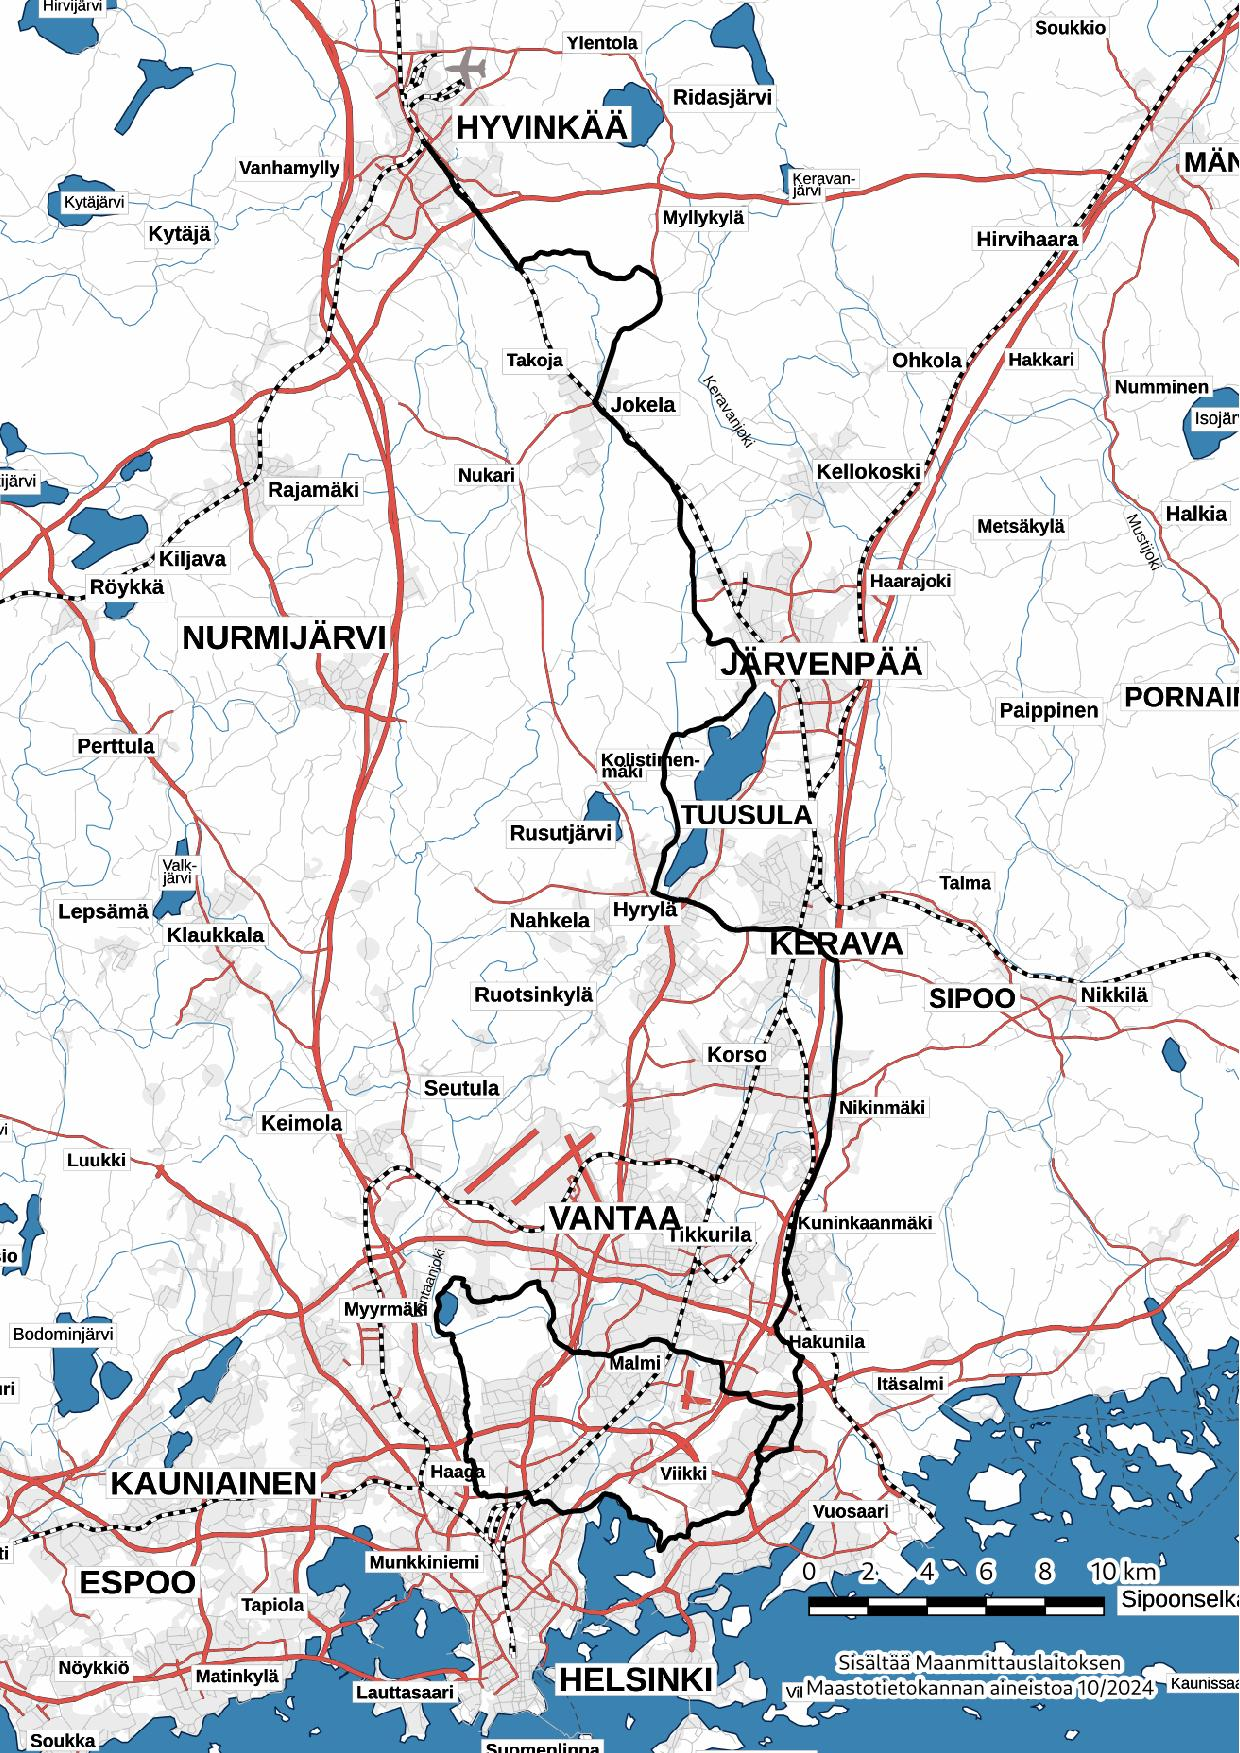
\includegraphics[width=\linewidth]{assets/mustaliljareitti.jpg}
\end{Figure}
\end{multicols}

\vspace*{.50cm}
{\raggedleft Teksti: Janne Suomalainen\par}
